% 标单百分号的注释,如本句所示。是原本模板注释
%%% 标三个百分号的注释,如本句所示。是辅助使用者理解的指导性演示,以“-BEGIN”与“-END”进行标记代码的起始位置和结束位置

%%% 与此同时,本文档作为包含子文件与分页符演示,其余功能演示内容详见 ./section/2.3.1_步兵机器人.tex 文档

% 引入导言区配置文件

%%% 包含子文件演示-BEGIN
% 文档全局设定与引入必要宏包

\documentclass[a4paper, twoside, zihao=-4, sub3section]{article}
\usepackage[hmargin=0.79in, top=0.95in, bottom=1.13in]{geometry}
\geometry{headsep=0.14in, footskip=0.47in}

\usepackage{pdfpages}
\usepackage{amsmath}
\numberwithin{figure}{section}
\usepackage{fancyhdr}

\usepackage{graphicx}
\usepackage{float}

\usepackage{ltxtable}
\usepackage{colortbl}
\usepackage{multirow}
\usepackage{graphicx}

% 字体配置

\usepackage[UTF8, heading=true]{ctex}
\setmainfont{Arial}
\setsansfont{Arial}
\setCJKmainfont[AutoFakeBold, AutoFakeSlant]{SimSun.ttc}
\setCJKsansfont[AutoFakeBold, AutoFakeSlant]{SimHei.ttf}

% 段落格式配置

\linespread{1.62}
\setlength{\parskip}{5pt}

% 目录配置

\usepackage[titles]{tocloft}
\usepackage{hyperref}
% 去除引用红框,改变颜色
\hypersetup{colorlinks=true,linkcolor=black}
% 重新定义目录的标题样式
\renewcommand*\contentsname{\hfill \color{black}\zihao{-2}\textbf{目录} \hfill}
% 设置点间距
\renewcommand\cftdotsep{0.1}
\renewcommand\cftsecdotsep{\cftdotsep}
\CTEXsetup[name={,.}]{section}
% 调节缩进
\setlength{\cftsubsecindent}{1em}
\setlength{\cftsubsubsecindent}{3em}
% 调节编号宽度
\setlength{\cftsecnumwidth}{14pt}
\setlength{\cftsubsecnumwidth}{20pt}
\setlength{\cftsubsubsecnumwidth}{30pt}
% 调节行距
\setlength{\cftbeforesecskip}{0pt}

% 标题配置

\usepackage{xcolor}
\newcommand{\titlecolor}{\color[RGB]{51, 51, 153}}
\usepackage{titlesec}
\titleformat{\section}
  {\titlecolor\zihao{2}\bfseries}
  {\thesection.}{0.5em}{}
\titleformat{\subsection}
  {\titlecolor\zihao{-2}\bfseries}
  {\thesubsection}{0.5em}{}
\titleformat{\subsubsection}
  {\titlecolor\zihao{3}\bfseries}
  {\thesubsubsection}{0.5em}{}
% 四级标题
\setcounter{secnumdepth}{4}
\titleformat{\paragraph}
  {\titlecolor\zihao{-3}\bfseries}
  {\theparagraph}{0.5em}{}

% 表格样式配置

\definecolor{tabhdcolor}{hsb}{0, 0, 0.72353}
\definecolor{gndcolor}{hsb}{0, 0, 0.96}
\AtBeginEnvironment{longtable}{\sffamily}
\renewcommand{\arraystretch}{1.1}
%%% 包含子文件演示-END
%%% 包含子文件,相当于把被包含的文件全部内容复制粘贴到此处
\usepackage{enumitem}
\usepackage{amssymb}
\usepackage{pifont}
\usepackage{graphicx}
\usepackage{array}
\usepackage{longtable}
\usepackage{tabularx}
% 文档内容-BEGIN
\begin{document}

    % 引入封面
    % 封面

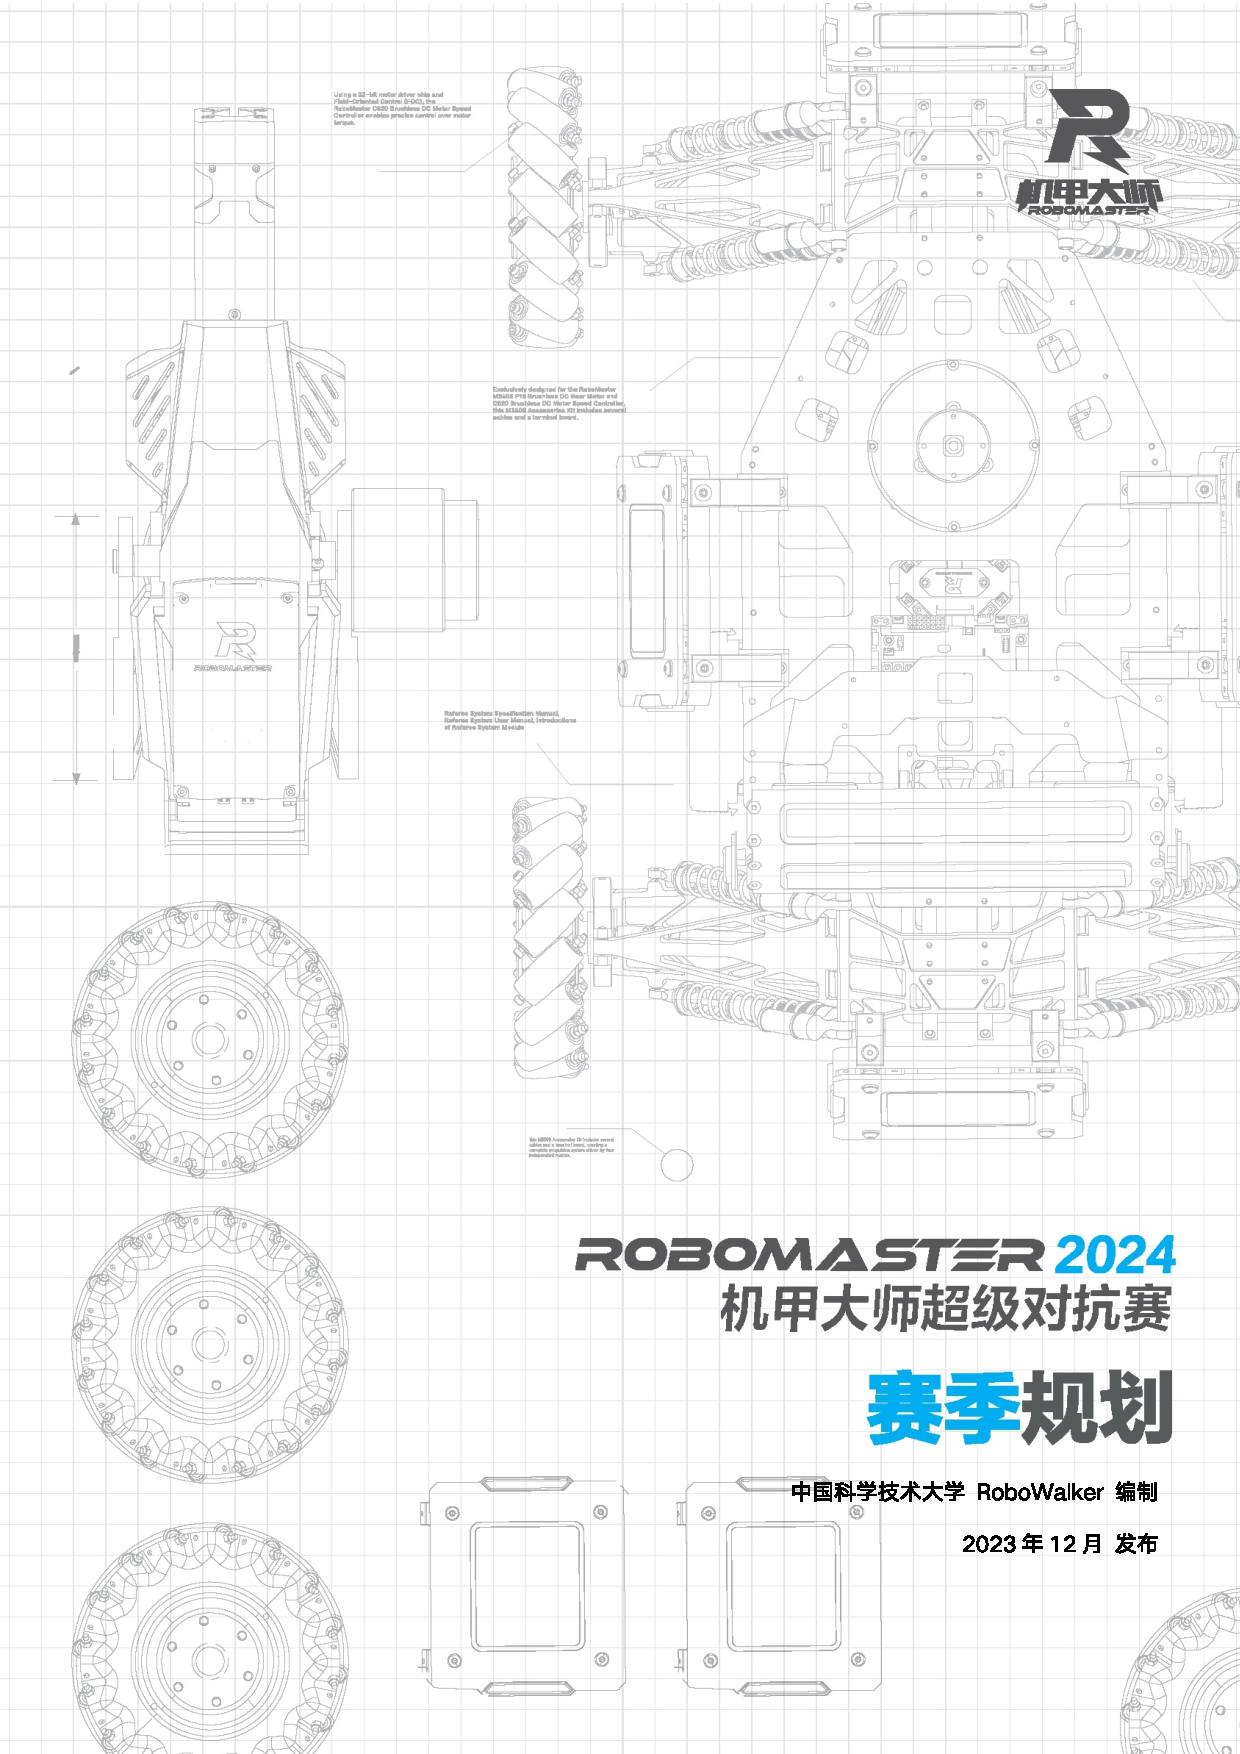
\includepdf{section/cover1.pdf}

% 编码页数从1开始
\setcounter{page}{1}

% 页眉页脚
\pagestyle{fancy}
\fancyhf{}
\fancyhead[EL, OR]{
  
\includegraphics[height=0.15in]{figure/header_img.png}
}
\fancyfoot[EL]{
  \zihao{-4}\thepage
  \hspace{0.4cm}
  \raisebox{.15ex}{
    \color{gray}{
      \zihao{-5}© 2024 \ 大疆创新 \ \ 版权所有
    }
  }
}
\fancyfoot[OR]{
  \raisebox{.15ex}{
    \color{gray}{
      \zihao{-5}© 2024 \ 大疆创新 \ \ 版权所有
    }
  }
  \hspace{0.4cm}
  \zihao{-4}\thepage
}

% 目录
\begin{center}
  \zihao{5}\tableofcontents
\end{center}

\newpage
    
    \section*{前言}

\addcontentsline{toc}{section}{前言}
    
    \noindent
    本报告由深圳技术大学悍匠战队编制,适用于RoboMaster 2025机甲大师超级对抗赛。主要撰写人员包括:
    
    \noindent
    \LTXtable{\textwidth}{table/0_writersList.tex}
    
    %%% 分页符演示-BEGIN
    \newpage
    %%% 分页符演示-END
    %%% 分页符,相当于从此处开辟新的一页,无论上一页内容是否凑够一页,都会从新的一页开始
    
    \section{团队目标}


    \subsection{团队目标概括}

        深圳技术大学悍匠战队始建于2019年,至今已有5年的备赛经验,自22赛季首次踏入超级对抗赛赛场后,均未能在区域赛的小组中出现,未能实现赛季成绩的进一步突破。\par
        对此,我们剖此往届赛季备赛中出现的管理和技术层面的不足之处,复盘反思与强队交手的经历,25赛季我们战队的比赛目标是晋级全国赛。\par
        为实现这个多年来的愿望,在25赛季中加强进度监管、在原有基础之上细微调整和优化、备赛过程中侧重于测试、进一步体系化传承资料和财务等各方面流程、引导队员探索技术背后的原理;加强队伍文化建设,提高队员比赛积极性和参与感,营造追求极致、患难与共的团队氛围,将生而无畏,精益求精的团队理念贯彻到每个战队成员。\par

        \subsubsection{团队实际情况}

            \paragraph{队伍可用资源}

                得益于学校和学院的大力支持,本赛季战队在资金、研发场地等方面比较充足。本赛季战队的资金来源主要有以下几个方面:上赛季剩余的耗材费、加工费等,2025年学院竞赛专项经费、实验室运行费用等多项经费约30万元。\par
                战队共有研发装配实验室3个,用于加工及物料存放的实验室1个,并配有一个约100平方测试场地可以放置1个联盟赛3V3对抗赛场地或1/4个超级对抗赛场地。\par
                战队拥有多台 3D 打印机,台钻,切割机,磨砂机等设备用于加工研发,拥有电子白板、打印机等设备满足队内授课、开会、成果展示等需求,配备了云台相机、单反相机、无人机等设备,能够满足战队宣传需求。此外通过老队员的资助实验室还配备了冰箱、制冰机等设施,提高队员生活质量。整体来看,我们战队的资源相对充足,能够满足战队的研发需求。\par
                目前我队拥有团队成员共 80 余人,根据我校课程设置、实习安排等实际情况,我们队伍的人员构成主要如下:大二队员是队伍的主干力量,需要完成本赛季各兵种的基础研发装配调试迭代工作,是比赛的主要参与者;大三与大四留队队员参赛经验较为充足,但因为自身学业与未来就业原因,偶尔会在队内对队伍进行指导,同时根据队员自身情况,进行相应技术点的研究与突破。大一队员作为梯队成员,经行比赛基础基础技能学习,完成各组队内考核的任务,进行各类基础模块建设与调试,同时为鼓励大一成员积极参与,研发创新,表现优异者可作为正式队员参赛。\par
                关于技术积累部分,经过上赛季的转变,传承下来的资料相较完整和体系化,在25赛季将继续推进各组文本、视频等形式的技术传承。我们队内主要的技术资源获取途径有邀请老队员回来对技术研究可行性分析、老队员留下的技术文档、公开的论文资料、工业界成熟的技术下放、组织与其他队伍的线下技术交流、RoboMaster论坛各队开源技术分享,以及各RM交流群的技术交流。\par

        \subsubsection{本赛季要完成的基础内容及进阶优化内容}

                经过过去几年各赛季的复盘和反思,历史的备赛策略过于激进、新赛季多次推翻旧赛季千辛万苦打下的基础,赛季初踌躇满志、备赛时忙不过来、缺乏明确的测试计划、赛场上稳定性欠佳。队员们普遍缺乏科学合理的设计和控制策略,这反映了主流的以项目驱动发展的学习路线无法兼顾犄角旮旯的知识空缺,队员们往往只能够解决具体的工程实践问题,而对技术背后的原理漠不关心,这是队员和队伍谋求长远发展无法忽视的阻碍。\par
                稳定性:在设计时,需要充分考虑模块的使用场景,在结构和配件材料选型上尽量做到合理;在装配时选择正确的零件,在交付下一环节前完成可用性和强度的检查,并及时记录缺陷以便于下一版本迭代;注意线路的布置合理与线束的物理保护,对可能磨损线材的地方加强保护,留下记录,并在下一版本设计上做出调整。此外,只有长期高强度的测试能够检验稳定性是否良好,在缺乏科学的分析能力的情况下也只有测试能够暴露出不稳定缺陷。\par
                设计指标与测试计划:在机器人研发的初始节点定下机器人性能指标并根据制定相应的调试测试计划,在队里进度管理系统中留下记录。测试也不止步于记录,需要将大量的测试数据汇总后分析成因。\par


            


    \subsection{各方向上的目标}

    \subsubsection{目标成绩}

        在比赛成绩上,由于我们战队已经有 5 次参加 RoboMaster 比赛的经验,并有两次成功参加超级对抗赛的经验,战队内经过全体讨论决定,本赛季希望能够进入全国赛。\par

    \subsubsection{任务进度管理制度}

        在赛季的各个阶段制定各兵种的整体任务进度安排,并将阶段性任务记录在飞书云文档,规定每个任务结束时间,每周定期由项目负责人核实验收上周任务完成情况并对遇到的问题进行总结并制定本周的工作安排,队长及项管参与每周各组工作安排会议,保证每个项目所需资源落实到位,进度情况健康。任务进度管理数字化记录,在项目管理系统上登记每周任务并实时更新任务状态,对进度情况不健康的项目做出及时调整。\par

    \subsubsection{队员管理制度}

        结合队员个人课程表情况对队员在实验室到岗研发时间有所要求,完善实验室考勤请假制度,考虑到学校人数越来越多,我们考虑对人员的要求要精益求精,整顿队风,对比赛参与度不高,研发积极性差,工作效率低效的队员作警告清退处理。同时提高实验室成员的责任意识,爱护实验室资产与环境,并制定了相应的奖惩制度,加强对梯队队员的培养。\par

    \subsubsection{物资管理制度}

        构建数字化流程化物资购买管理制度,增强对物资购买的流程审核及记录,提高现有资源利用率,减少不必要的浪费,对高价值物资如电机进行出入库登记处理,物资领用责任到人,对于由于低级错误或者恶意损坏物资的成员实行罚款制度。\par

    \subsubsection{新人培养体系}

        构建数字化流程化物资购买管理制度,增强对物资购买的流程审核及记录,提高现有资源利用率,减少不必要的浪费,对高价值物资如电机进行出入库登记处理,物资领用责任到人,对于由于低级错误或者恶意损坏物资的成员实行罚款制度。\par

    \subsubsection{管理流程改变}

        本赛季的管理方式继续沿用上赛季队长,项管主导项目方向,各技术组组长评估技术可行性,各车组负责人主导研发方向的形式,主要流程为:队长项管制定各车组的需求,技术组长分析技术可行性,的出最终需求结论,由车组负责人制定研发方向,再由技术成员讨论技术细节。\par

    \subsubsection{技术传承建设}

        在研发调试过程中遇到缺陷或陷阱及时记录,撰写“警钟长鸣”文档,对每个新研发的技术点留下相应的技术文档。在赛季结束都需要撰写自己负责部分的技术文档(包括已实现的技术细节和未实现的预研资料),安排相关负责人跟进文档进度。\par

    \subsection{技术突破}
    
    \newpage
    
    \section{复盘分析}

    \subsection{整体分析}

    上一赛季的对抗赛我们的队伍未出线,成绩不理想,但相较于更早些时候的失败,机器人的性能有显著上升,稳定性仍然欠佳。\par
    整体而言上个赛季备赛过程中出现的错误以及进度落后归根结底是赛季初的决策失误导致的,在赛季初不应当因为经济富余、时间充分而采取极端激进的备赛策略,应当量力而行,建立在上一赛季的基础之上维护、测试、优化,循环往复,在进度稳定推进之余尝试创新或接纳新技术。\par
    在新赛季,我们将着力于测试开发、对机器人进一步迭代和优化,继承原有基础,深入学习钻研应用广泛的通用技术,同时积极推动新技术的研发、丰富技术储备。\par

    \subsection{上赛季各项目组问题和挑战}

    \paragraph{机械组}

        \setlist[itemize]{label=\raisebox{-1.2ex}{\scalebox{3}{$\textbullet$}}}

        \begin{itemize}
            \item 上赛季机械组的主要问题为技术传承与研发进度。由于传承管理问题,老的上场车辆未能得到留存,使得上赛季各车组的机械结构几乎都是从零做起,在根本上影响了研发进度,造成技术断代。
            \item 且上赛季各车组机械结构有较大变化,使得研发任务较重,一定程度上也影响了进度。进度的滞后也使得后续测试时间严重不足,导致车辆稳定性完全不足以支撑三场比赛。
            \item 上赛季由于进度安排和技术传承的问题导致机械组成员在技术上无力深度钻研,延续至25赛季暴露出了机械组成员缺乏理论支撑和系统的分析方法的新问题,导致技术难以短期实现突破。
        \end{itemize}

    \paragraph{电控组}

        \setlist[itemize]{label=\raisebox{-1.2ex}{\scalebox{3}{$\textbullet$}}}

        \begin{itemize}
            \item 上赛季电控组的最大问题在于进度把控上,各兵种机器人的测试时间最短的只有一两周,测试不足导致部分问题没能在赛前测试阶段检查出来,从而导致赛时各兵种机器人的总体表现不稳定。
            \item 其次是新人流失问题,在新人培训结束后出于各种原因未能及时给新人布置任务导致新人长期处于无事可做的状态,而且新人缺乏引导,不知道有什么事情可以做,导致新人的贡献度很低,第一批入队的新人流失了一半有余。
            \item 电控方面同样出现了与机械组类似的“技术空心”问题,队员更倾向于项目驱动的发展路线,在过去的一个赛季中培养起了项目实践和解决实际问题的能力,但普遍缺乏对理论知识的钻研精神,后续将有引导性地安排任务。
            \item 由于上述缺陷,导致平衡步兵的技术传承进展比较困难,进而导致新老队员在技术认知上产生分歧、爆发矛盾。
        \end{itemize}

    \paragraph{视觉组}

        \setlist[itemize]{label=\raisebox{-1.2ex}{\scalebox{3}{$\textbullet$}}}

        \begin{itemize}
            \item 由于没有自适应弹道校正,弹道需要手动调整。然而很多时候发现场外测好的抬枪补偿数据,在场内不适用,出现打偏的情况。每次比赛都要测试抬枪补偿的流程过于繁琐和着急,而且场外空间很有限,十分不便。
            \item 哨兵缺少初始位姿校准流程,导航路线会向一个方向偏移;自瞄时云台抖动严重.
            \item 视觉组在上个赛季中暴露出人手严重不足的问题,甚至需要一名视觉组成员负责维护多个兵种,初步认为是算法学习周期长、学习成本大导致的,而且学习期间很难参与机械和电控的进度,导致后期视觉新人无法融入集体、被边缘化,最后人员流失。25赛季中以兵种为单位分配工位、鼓励视觉组新人参与实验室相关活动、进一步加强算法传承、老人带领新人参加其他比赛练手等措施。
        \end{itemize}

    \paragraph{硬件组}

        \setlist[itemize]{label=\raisebox{-1.2ex}{\scalebox{3}{$\textbullet$}}}

        \begin{itemize}
            \item 在上一赛季中,硬件组遭遇了新成员参与度不足的问题。根源在于开展了周期过长的培训工作,新成员在赛季中期尚未完全融入团队的日常调试和维护工作,导致人手短缺,影响了团队的整体运作效率。
            \item 此外,新老技术传承与交替的过程中出现了问题,在备赛中期出现较长时间的技术断层。
            \item 上个赛季中队伍整体的硬件需求局限于超级电容的开发与维护,碍于超级电容的学习成本,新人难以参与其中。25赛季中整体队伍对硬件的需求陡增,反而导致硬件组人力短缺的情况,在招新中将硬件组独立于电控组招揽新人。
        \end{itemize}

    \paragraph{运营组}

        \setlist[itemize]{label=\raisebox{-1.2ex}{\scalebox{3}{$\textbullet$}}}

        \begin{itemize}
            \item 在财务管理方面,由于比赛周期长、投入大,战队面临着资金筹集与合理分配的巨大压力。一方面,运营组需要积极寻求学校支持,确保战队能够持续运转;另一方面,又要精打细算,对每一笔支出进行严格审核,确保资金用在刀刃上,如耗材采购、日常运营等,这对成员们的财务规划能力提出了极高要求。
            \item 在周边设计方面,运营组旨在通过创意周边产品增强战队影响力和团队凝聚力。然而,如何在体现RoboMaster赛事文化的同时,又能贴近大学生群体喜好,设计出既实用又具有吸引力的周边,成本控制与生产效率的考验让战队在设计、生产过程中必须再三权衡。
            \item 在宣传方面,如何在众多参赛队伍中脱颖而出,有效传达悍匠战队的技术实力、战队理念及比赛亮点,是一项不可小觑的任务。运营组不仅要策划并执行多渠道的宣传工作,还要应对内容同质化等挑战。
            \item 在25赛季中主要由管理层优化运营组工作流程来减轻运营组成员的压力,例如将财务压力部分分摊到项管、技术组组长上,优化采购流程;另一方面给运营组提供足够的资源支持其带领技术组成员参与其他比赛,并以此为亮点吸引组织外的运营人才参与比赛和转化为运营组成员。
            \item 在设计方面,广泛汲取其他队伍的优秀设计经验并结合队员的审美偏好设计有创意、实用或有吸引力的周边。
        \end{itemize}

    \subsection{上赛季的成功方面}

    \subsection{根因分析}

    \subsubsection{问题分析}

    \subsection{问题解决方案}

    \setlist[itemize]{label=\raisebox{-1.2ex}{\scalebox{3}{$\textbullet$}}}

    \begin{itemize}
        \item 增加测试频率和测试强度,总结出适应各个兵种的测试方案和测试流程。
        \item 在赛季中后期组织队内3V3,尽可能模拟赛场实况,培训操作手。
        \item 倾注更多人力物力投入远程击打兵种。
        \item 活跃实验室气氛,充分沟通交流,打通队内信息差。
        \item 硬件组独立招新、培训。
        \item 将主力开发的工位安排尽可能集中,便于了解各兵种进度。
        \item 优化物资采购,改为由组长审核、分批次购买,通过其他赛事吸引运营人才。
        \item 举办校内赛,鼓励新人参与实验室事项。
        \item 制定一套详细的赛前维护。
        \item 实现弹道自动校正。
    \end{itemize}

    \subsection{上赛季经验总结}

    \newpage
    
    \section{项目分析}


    \subsection{新赛季规则解读}

    \subsubsection{整体规则分析}

    \subsubsection{比赛机制调整}

    \subsubsection{场地调整}

    \subsubsection{各兵种规则分析}

        \paragraph{步兵规则分析}

            \setlist[itemize]{label=\raisebox{-1.2ex}{\scalebox{3}{$\textbullet$}}}
    
            \begin{itemize}
                \item 25赛季可在准备3分钟内预装弹,且不再限制初始预装弹数量,根据以往比赛经验,要求步兵机器人至少拥有400发的预装弹量。本赛季现有设计中,步兵机器人预装弹量已满足要求,但机械组仍需尝试在不牺牲其它性能的前提下继续扩大预装弹量。
                \item 25赛季步兵通往关键交战区中央高地共有四条可选路径:翻越小资源岛台阶、公路区、公路隧道、高地隧道。由于普通步兵不具备翻越台阶的能力,故小资源岛台阶不予考虑;公路区与公路隧道需要经过颠簸路段,且公路区路程较长,考虑25赛季新增使用能量总额限制(20000焦),为减少功耗,普通步兵在非必要情况下应避免选择这两条路径;高地隧道路程短且无需经过颠簸路段,是普通步兵出入中央高地的最佳路径,因此本赛季普通步兵机器人必须具备穿越隧道的能力,这就要求机械组必须设计出尺寸合适,能够穿越隧道的机器人。此外,步兵可通过飞坡直达敌方公路区,从而阻击敌方英雄吊射以及快速接近敌方基地区,这要求本队步兵机器人机械组必须研发出重心适中,具备稳定飞坡能力的步兵机器人。
                \item 相较于24赛季,平衡步兵的概念以及经验加成等规则红利被取消,归类到普通步兵,从前后两块大装甲板变为了四块小装甲板,更容易被对方机器人打击,看似轮腿步兵相对于普通步兵毫无优势,但因为其功率计算的特殊性,使得它能够在一个较小的功率内仍有较快的移动速度,进攻、回防速度快,同时可以限制对方英雄吊射;并且五连杆机构给予了轮腿步兵很强的灵活性,能够轻松通过起伏路段,实现蹭台阶和飞坡等地形跨越动作来获得地形跨越增益,因此轮腿步兵在比赛中应该充当速攻、抢点、回防的角色。
                \item 25赛季堡垒增益点仅在己方前哨站被击毁,且基地血量落后时生效,可被一台哨兵或步兵占领,获取无敌、枪口热量、发弹量等增益,在防守基地区时拥有巨大优势。当基地区遭到入侵且哨兵不能优先占领堡垒点时,步兵应积极占领堡垒点。
                \item 25赛季能量机关可由任意机器人激活,但出于经济考虑,激活能量机关的最佳选项仍是机动性最高的步兵,此外,激活能量机关后会为基地和前哨站带来防御增益,为机器人带来攻击增益,使得队伍更容易展开进攻或进行防守,因此能量机关的激活将是本赛季的重中之重。
                \item 25赛季步兵机器人仅靠发射弹丸、或在 3 分钟内对前哨站造成 500 点伤害、或成功击打对方机器人所带来的经验值是不足以升级的,这要求步兵机器人在本赛季要做到快速精准的打击,并与队友制定相关战术策略以更快提升等级。进攻时,步兵机器人应积极占领中央高地区域,为己方英雄和步兵带来增益,对对方机器人造成更有力的打击,防守时积极占领堡垒、前哨站和基地区,获取防御增益进行反击。
                \item 对于轮腿步兵,除上述占领增益点外,还能在飞坡点和公路区地形跨越增益点进行交互获得增益,因此要求电控的算法要具备很强的稳定性。
                \item 操作方面,25赛季与24赛季一致,可选择手动控制或半自动控制。半自动控制相比24赛季,增加了25\%的防御增益。半自动步兵在数值上将会比手动控制步兵有更大的优势。	
                \item 25赛季新增底盘能量总额20000焦限制,一旦超出限制,则机器人的功率永久削减,因此,本赛季应制定能量使用策略,减少非必要的能量消耗。
            \end{itemize}
        
        \paragraph{步兵策略战术}
    
            \setlist[itemize]{label=\raisebox{-1.2ex}{\scalebox{3}{$\textbullet$}}}
    
            \begin{itemize}
                \item 步兵在具有高机动性和灵活性的同时,对前哨站和基地的伤害收益小,且血量较少,因此步兵在比赛中的主要职能为占领增益点、掩护和支援我方其它机器人单位、阻击敌方英雄、攻击敌方地面机器人以及协同激活能量机关。
                \item 在开局针对中央高地的争夺战中,轮腿步兵因为功率计算和五连杆机构的特殊性,具有较强的机动性,可以通过蹭台阶迅速占领中央高地增益点并对对方机器人进行打击,同时,我方步兵应当尽量避免进入敌方哨兵的索敌范围。
                \item 当己方英雄吊射命中率较高时,步兵优先选择掩护英雄,防御敌方飞坡步兵;当英雄吊射命中率偏低时,选择从香蕉道到对方区域干扰敌方英雄吊射(具体能否实现需要看最终的尺寸),以及攻击敌方地面机器人。
            \end{itemize}
    
            \begin{figure}[H]
                \centering
                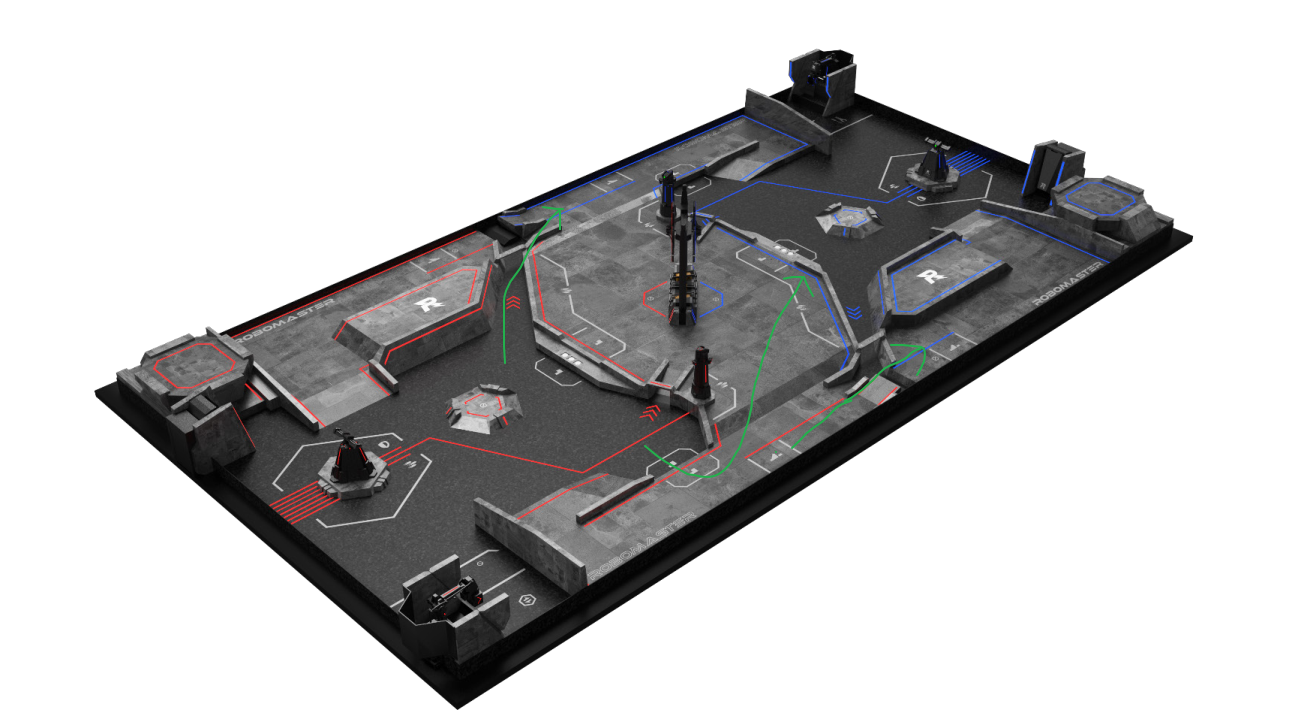
\includegraphics[height=0.35\textwidth]{figure/infantry_tactics.png}
                \hspace{0.5em}
                \label{fig:infantry_tactics}
            \end{figure}

        \paragraph{英雄规则分析}

            \setlist[itemize]{label=\raisebox{-1.2ex}{\scalebox{3}{$\textbullet$}}}
    
            \begin{itemize}
                \item 今年的英雄机器人引入了“部署模式”,在己方半场内,英雄机器人可通过2秒的确认时间进入“部署模式”,底盘断电后获得25\%的防御增益,并获得狙击攻击增益与经济加成。这一机制的引入,英雄在己方半场的任意位置,对敌方基地造成可观的伤害输出。“部署模式”需要其他兵种的协同支持,为团队协作和战术规划提供了更多可能性。同时规则对适用于部署模式的“比赛节奏”做出了一些限制,开局有2次命中能享受部署模式加成,此后每20s增加一次机会。
                
                \item 今年新增的42°坡提升了地形复杂度,对英雄机器人的底盘设计和功率分配提出了全新要求。传统的麦克纳姆轮加上英雄机器人的重量难以胜任这一高难度场景,地形上鼓励其他底盘结构(例如舵轮底盘)。42°坡本身是一个极具战略价值的狙击点,占领这里可以对战局产生重要影响。同时这一位置容易受到对方无人机的威胁,对时机的精准把控至关重要。解决这些技术难点,我们就能在比赛中抢占先机,充分释放英雄机器人的潜能。
                
                \item 能量体系:今年的规则更新中,英雄、步兵、哨兵机器人在底盘能量消耗达到20000J后将进入“虚弱”状态,对于比赛节奏和战术规划有新的要求。这一规则也对电容的性能和整车的能量控制系统提出了更高要求。如何提升电容效率、优化整车能量管理,将成为提高胜率的关键技术突破点。
                
                \item 赛制时间分析:在新赛季中,空中支援机制进行了调整,英雄在前30秒需要占领梯形高地、准备击打前哨站,30秒后将与无人机和对方英雄机器人形成制约。地形变化使得梯形高地的防御增益对英雄机器人的吊射和部署模式至关重要。若某方的梯形高地增益点仅被该方机器人占领,则在比赛的不同时间段(2-3分钟、3-5分钟、5-7分钟),占领的机器人可获得2、3、5倍的枪口热量冷却增益和25\%的防御增益。
                
                \item 雷达机制分析:雷达可以向所有己方机器人发送数据,接收哨兵机器人的数据。新规则下英雄吊射点位更加灵活,但在部署模式下底盘处于“失能状态”,此时很容易陷入被动。对于吊射点位的选择,可以通过感知敌方位置,为英雄操作手实时更新可以进行吊射的位置;或直接检测预设的吊射点位是否有敌方单位,方便操作手进行决策,提前预警,减少被抓风险,提高灵活性。还能在敌方进入基地范围内时,向英雄操作手发送”防守”的决策信号,调动英雄回防。
    
                \item 英雄狙击模式下,命中敌方基地会获得50金币。英雄狙击伤害可获得100经验值,跟上赛季一样,但是区别在于这赛季英雄新增的部署模式,可以随时狙击。也就是说英雄如果能利用好这个狙击能大大增长升级速度,同时前期也可以使用狙击击打较好命中的目标,加速升级。
    
                \begin{figure}[H]
                    \centering
                    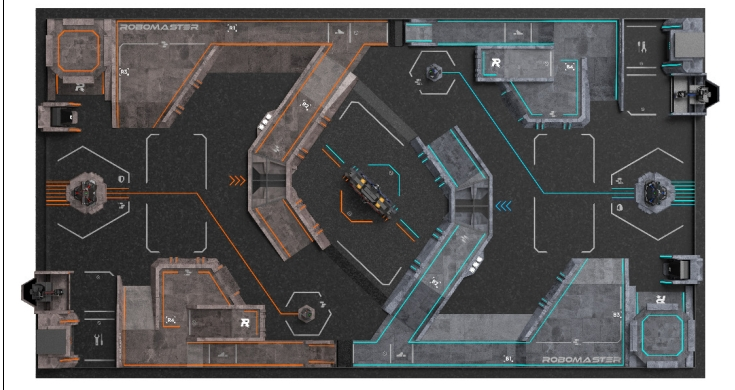
\includegraphics[height=0.35\textwidth]{figure/RM2024_map.png}
                    \hspace{0.5em}
                    % 添加居中、黑体、加大的字体
                    \caption{\textbf{\zihao{-4}\textbf{RM2024场地示意图}}}
                    \label{fig:RM2024_map}
                \end{figure}
                
                \begin{figure}[H]
                    \centering
                    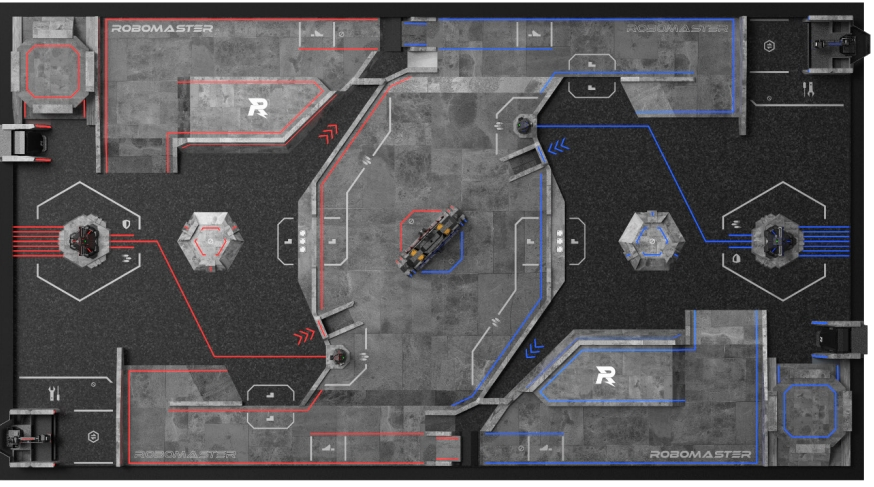
\includegraphics[height=0.35\textwidth]{figure/RM2025_map.png}
                    \hspace{0.5em}
                    \caption{\textbf{\zihao{-4}\textbf{RM2025场地示意图}}}
                    \label{fig:RM2025_map}
                \end{figure}
    
                \item 场地中央的环形高地更换为中央高地,进入中央高地的路径也完全更改——24赛季可以由基地区直冲环形高地,但25赛季将公路区和中央高地直接连接,阻断了基地区直冲中央高地的行为,影响了英雄机器人冲锋的效率。并且中央高地和梯形高地改动,导致飞坡后英雄的路线选择减少,加大了飞坡的风险,由此可能要重新考虑飞坡的进攻价值性。
    
                \item 而中央高地的20°坡、狗洞和弯曲的香蕉道狭道,对于目前战队的英雄机器人而言是无法通过的,战略意义不大。如果后续场地不加以大的改动,可以尝试制造一台超小英雄过此类狭窄通道。
    
                \begin{figure}[H]
                    \centering
                    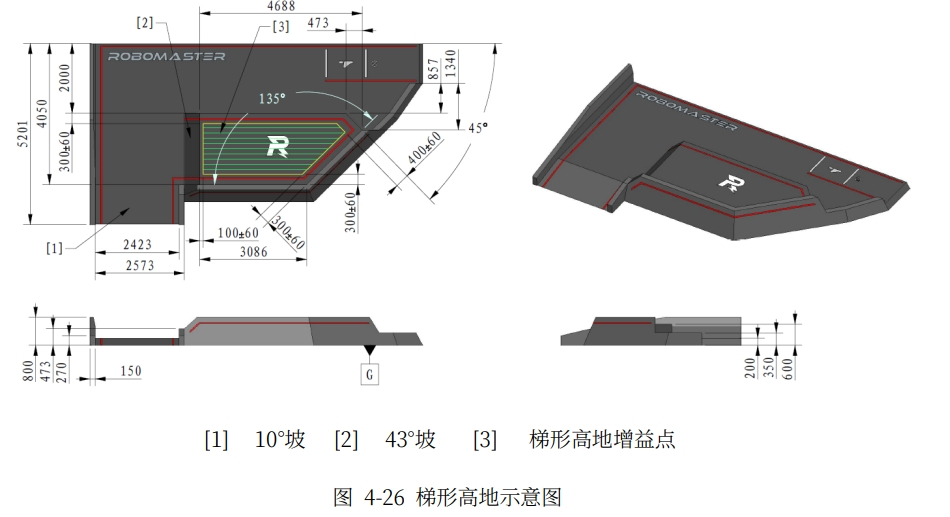
\includegraphics[height=0.35\textwidth]{figure/trapezoidalElevation.png}
                    \hspace{0.5em}
                    \caption{\textbf{\zihao{-4}\textbf{梯形高地场地示意图}}}
                    \label{fig:trapezoidalElevation}
                \end{figure}
    
                \item 梯形高地最受瞩目的就是43°高地,600cm的高度让能够上到这个高地的英雄机器人安全性得到了保障,目前看来所有兵种之中对在高地上有较大威胁的是平衡步兵和无人机。此高地还是全场中最适合吊射基地的位置,且距离前哨站只有7~8米的距离,还没有任何的障碍物遮挡视野。可以说,它就是提供给英雄的专属发射场地,重要性不言而喻,所以己方梯形高地是英雄前期必须尝试占领的战略要地。在前哨站失守的中期焦灼阶段和后期进攻阶段都可以尝试飞坡占领敌方梯形高地,为英雄自己创造一个较为安全的输出基地环境。但实现上坡对于英雄机器人的性能有一定要求,不管是轮毂影响,还是整个底盘通过角和重心位置设计,对于每一个队伍都是一个大的挑战。
                
                \begin{figure}[H]
                    \centering
                    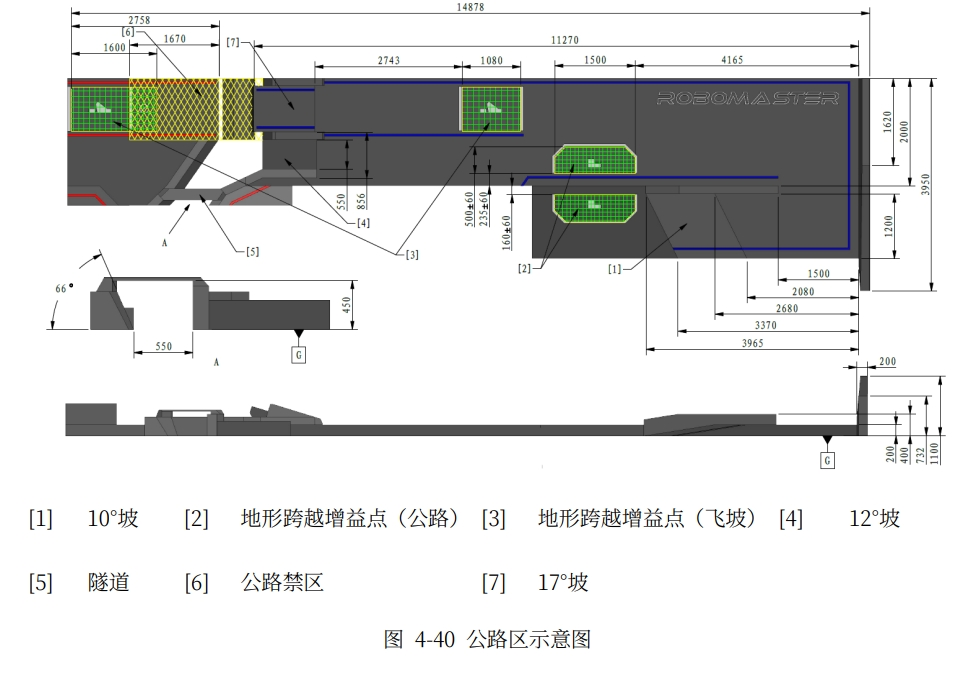
\includegraphics[height=0.35\textwidth]{figure/highwayArea.png}
                    \hspace{0.5em}
                    \caption{\textbf{\zihao{-4}\textbf{公路区场地示意图}}}
                    \label{fig:highwayArea}
                \end{figure}
    
                \item 直角弯对英雄机器人的转弯性能提出较高的水平要求,虽然在机械结构上麦轮底盘和舵轮底盘是可以通过,但对于操作手来说需要有熟练的操作才能减少过弯时间,避免磕碰,提高进攻效率。飞坡区域直接衔接到敌方梯形高地,并且只有梯形高地一条路可以走,一旦被敌方察觉并派遣机器人堵在梯形高地的出口,那么飞坡过去的英雄只能被瓮中之鳖,除非明确知道敌方所有机器人分布位置。在战略规划上,若非紧急情况不推荐英雄飞坡,但在功能规划上,英雄要具备飞坡功能。在通过与中央高地衔接部分和香蕉道的上坡部分,英雄机器人需要注意的是在进攻时段是否有敌方的步兵机器人存在,进攻或撤退时需要保证自身安全,此外没有任何其他过多要求。
    
    
                \begin{figure}[H]
                    \centering
                    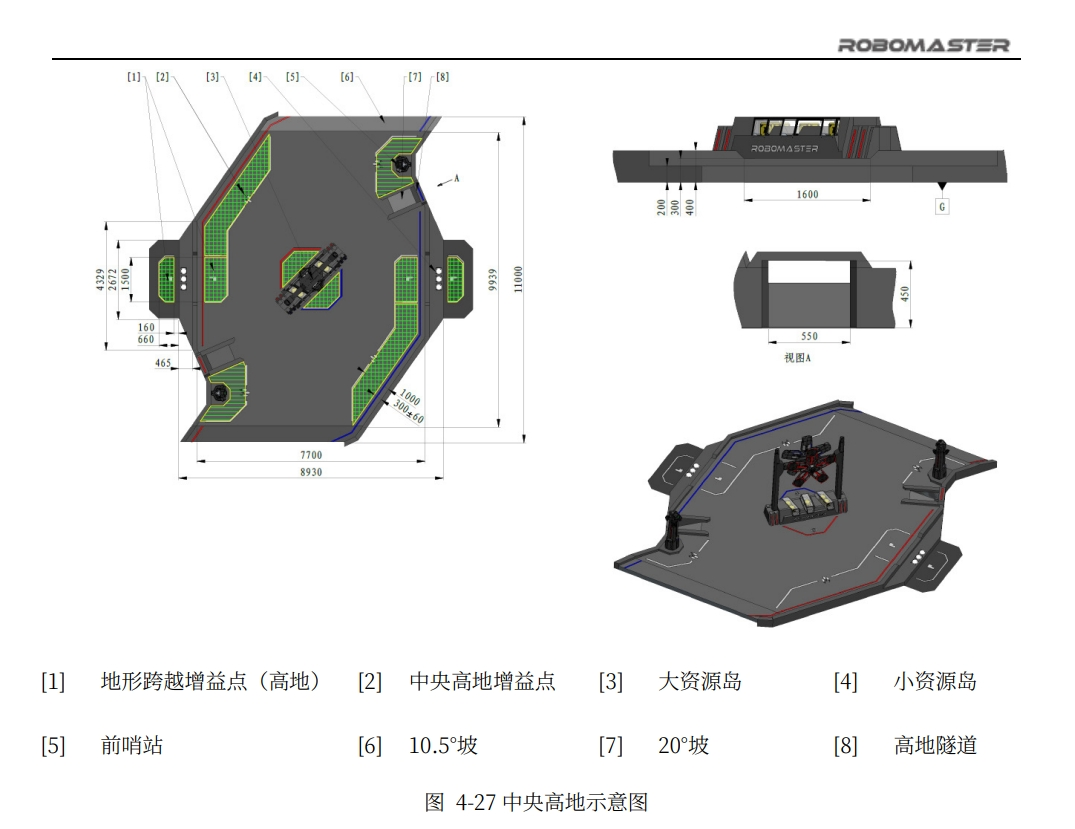
\includegraphics[height=0.35\textwidth]{figure/centralTableland.png}
                    \hspace{0.5em}
                    \caption{\textbf{\zihao{-4}\textbf{中央高地场地示意图}}}
                    \label{fig:centralTableland}
                \end{figure}
    
                \item 关于中央高地英雄机器人需要注意的就是颠簸路段、敌方“香蕉道”入口、狗洞以及敌方公路区出口。对机器人在性能有较高要求的就颠簸路段,在机器人制作中需尽量减少颠簸的影响性,但在多年比赛的经验来看,过颠簸路段时,无法发射,无法防御,只能快速通过,不然只能当活靶子。当英雄机器人在中央高地的时候,一定要时刻注意背后的香蕉道入口,中央高地四通八达,前后都有可能面临来敌。
    
            \end{itemize}

        \paragraph{英雄策略战术}

            \setlist[itemize]{label=\raisebox{-1.2ex}{\scalebox{3}{$\textbullet$}}}
    
            \begin{itemize}
                \item 出门左拐就是梯形高地了,英雄在比赛开始后可以尝试站住,攻击敌方前哨站,并为己方提供对于中央高地的态势感知。在设想中,梯形高地的落差同时也可为英雄提供对低处攻击的掩蔽,因此这里应该是英雄经常来的地方。
                \item 部署机制以底盘断电为代价换取一系列加成,虽然此时英雄有25\%防御增益,但在潜在的陆空威胁下仍十分脆弱。在地形复杂且四通八达的环境下,要求己方为英雄构建安全的“堡垒地带”显然难度较高,为此英雄操作手应该留意敌方无人机与地面机器人的出动与补给节奏(后半场可能的充电高峰期),见缝插针地抵近输出敌方前哨站与基地,并在危险来临时及时转入防守。
                \item 虽然组委会提过会增加飞坡之后的可选路径,但目前跨过沟壑之后,撤退的路径会经过敌方堡垒区,极有可能一去不复还,从敌方的角度而言飞坡的风险增大了不少。但同时加高的梯形高地也为到达敌方半场的机器人提供了更好的掩体。如果是快结束了想放手一搏可以考虑考虑。
                \item 无论是爬坡上梯形高地还是绕道己方公路区前往中央高地都势必会消耗不少能量,因此英雄应精打细算,增大补给间隔,并在比赛进行到下半场时择机在补给区“充电”。
                \item 对于底盘能量20000J的分配,前期应集中在占领梯形高地,中期寻找不同的部署点攻击对方基地,后期则需退回基地区拦截敌方步兵和英雄.
            \end{itemize}

        \paragraph{哨兵规则分析}

            \setlist[itemize]{label=\raisebox{-1.2ex}{\scalebox{3}{$\textbullet$}}}
    
            \begin{itemize}
                \item 哨兵在这个赛季的机制改动相当大,主要的改动在于哨兵取消了与前哨站挂钩的无敌机制、哨兵与比赛胜负的判定机制以及哨兵巡逻区的取消。此外,哨兵的初始发弹量也从400发削减到了300发,而且虽然底盘功率上限未做改动,但是哨兵和步兵、英雄一样适用于全局20000J底盘总能量的约束。这些改动无疑削弱了哨兵的单兵作战能力,也进一步提高了哨兵对完善的导航避障、自身定位、全局规划、灵活决策、资源调度和与其他机器人打配合的需求。
                \item 哨兵在这个赛季的战场上也依旧存在着不小的优势:首先,这个赛季并未对哨兵的枪口热量上限、每秒冷却做改动,这保证了哨兵在可发弹量充足的情况下输出能力依旧恐怖,而且,每一分钟哨兵都可以通过导航到补给区补血补弹或者远程兑弹的方式补充发弹量,这些机制平衡了哨兵初始发弹量削减的影响,在导航完善和工程获取经济能力强的情况下哨兵的发弹量甚至可能只取决于预装的弹丸有多少;其次,哨兵虽然取消了与前哨站挂钩的无敌状态,但是初始数据400血量100功率上限(步兵满级数据)保证了哨兵前期的性能和生存能力在线,配合恐怖的火力,在前期哨兵在面对对面的地面输出单位是具有绝对的压制力的,而且哨兵可以远程兑换血量以及它的复活机制并未改变,这意味着原本弹尽粮绝、性命垂危的哨兵可能突然以一个较好的状态重返赛场,对敌方形成巨大的威胁;况且,这个赛季新增了哨兵可以占领的堡垒增益点,当堡垒增益点开启,哨兵占领之后依旧可以获得无敌、额外发弹量和额外的枪口冷却增益,这一改动大大增强了哨兵的防守能力。
                \item 这个赛季的机制变动使哨兵更加全能,不论是在进攻端还是在防守端都有着独特的优势。显然,本赛季的改动无疑是令哨兵机器人的技术栈更加接近于全自动机器人的本质。没有一个完善的决策体系的话,在全局资源的规划和调动上会出现不可忽视的问题;巡逻区的取消无疑是对哨兵如何及时的规划进攻和回防路线将会是导航和定位上的挑战。
            \end{itemize}

        \paragraph{哨兵策略战术}

            \setlist[itemize]{label=\raisebox{-1.2ex}{\scalebox{3}{$\textbullet$}}}
        
                \begin{itemize}
                    \item 哨兵的前期作战能力是所有地面机器人中最强的,在前期利用高性能迅速占领中央高地上的增益点的战术价值很高,不论是前压前哨站还是阻击对面攻势都会令对手很头疼。
                    \item 哨兵可以在能量机关激活的时候击打能量机关获得额外增益。
                    \item 哨兵能远程补弹,可以在自身增益足够高或敌方状态差时乘胜追击,或是在被动防御时 尝试突围、扭转局势。
                    \item 哨兵可以通过雷达通讯接口得到鸟瞰全局的数据,通过自主决策可以选择进攻、防守、配合其他机器人或者规避围剿。
                    \item 哨兵可以占据中央高地,对靠近高地的机器人进行阻击和对取矿的工程机器人进行拦截。
                    \item 哨兵能接收云台手发送指令,在必要的时候可以解决一些意料之外、情况紧急的情况。
                \end{itemize}

        \paragraph{工程规则分析}

            \setlist[itemize]{label=\raisebox{-1.2ex}{\scalebox{3}{$\textbullet$}}}
    
            \begin{itemize}
                \item 小资源岛变更:小资源岛依旧紧贴中央高地护栏外侧,但银矿由原来的半嵌入式改变为完全嵌入,从原来可以通过夹爪直接取出改变成要求工程机器人从上面将其拔出,对工程机器人的机构要求更加灵活。
                \item 前往资源岛的路径变更:原来前往大资源岛的路径可以通过前哨站然后直接登上大资源岛或者直接钻隧道,而25赛季登上大资源岛的路径更加灵活,在基地正方向新增一个高300mm的二级台阶,第一级是高为200mm的小资源岛,所以工程机器人可以设计一个灵活的机构来完成登岛直接抵达大资源岛,而且现在是公路区连接着中央高地,所以工程机器人也可以选择绕远路先通过公路区再上岛,而上公路区又有选择,可以通过上200mm高的台阶进入公路区,也可以通过爬10°坡上公路区进而前往大资源岛,所以工程机器人的构型可以有更多选择特别是在底盘上。
                \item 经济体制改变:删除了五级难度的兑矿等级,等比例增加了剩余难度等q级的金币数量,且比例提高了随着兑矿次数增多时最低可选择兑矿难度的金币倍率,且新增选择四级难度时,工程机器人需要在15秒的时间限制内,连续兑换2块矿石,若在时限内兑换成功,2块矿石的所得金币将依次连续结算,否则将不会获得任何金币的机制,这需要工程机器人需要有非常灵活的兑矿机构,且操作手需要对操作更加熟练。 
            \end{itemize}

        \paragraph{工程策略战术}

            \setlist[itemize]{label=\raisebox{-1.2ex}{\scalebox{3}{$\textbullet$}}}
    
            \begin{itemize}
                \item 工程机器人定位:根据 25赛季规则的改动,我们认为工程机器人在25赛季的定位更加 偏向于通过取矿-兑矿换取金币达到为团队提供经济的一个角色,为其他车组提供更好的 配置条件,为多样化的战术选择提供经济支持。
                \item 取矿机构:六轴机械臂+吸盘。考虑到维修成本和迭代的选择上,使用板材替代上届的机加工方案。同时考虑到6r型机械臂Link1和Link2电机的承重,决定在这两个关节中引入弹簧的重力补偿,去避免电机的发热,延长使用寿命。
                \item 底盘选择:月球车底盘。由于场地的变更,工程机器人可以选择跨台阶的方式直接登上大资源岛,为了更快的争夺金矿来提高团队经济,我们选择可以适应复杂地形的月球车底盘来实现跨台阶的目标,在轮组的选择上我们将采用麦克纳姆轮来实现底盘的转向。 抬升兼存矿机构:剪式抬升架+一键2/3银矿.
                \item 抬升架的选择:剪式抬升。由于六轴机械臂的操控,我们采用剪式抬升架来抬升,并且在上面安装取银矿机构,使得可以取2/3个矿,由规则手册中场地部分可知,每两个银矿的中心距离为270mm,一键3矿则需要540mm,是可以尝试并且完成的(就怕后面又改规则),同时银矿一开始距离地面200mm,完全抽出来则需要400mm,所以会做一个180度的翻转使其更加稳定并且为后期存矿做足准备。
                \item 自定义控制器:带有六个角传感器的大臂缩小机械臂,采用大臂构型缩小的自定义控制器,有利用操作手更加直观的操作机械臂的运动,并同时减少解算需求,并考虑在自定义控制器中融入移动、吸取等快捷功能,以提升工程在存取矿的能力。
                \item 上位机实现:上位机采用ros2和movelt,将实时获取大臂的六个角度并跟踪机械臂的构型,在需要存取矿时,上位机将实现一次性取矿的路径规划。
                \item 下位机:优化各部分通讯,尝试在下位机实现机械臂正逆解算。
            \end{itemize}

        \paragraph{飞镖系统规则分析}

            \setlist[itemize]{label=\raisebox{-1.2ex}{\scalebox{3}{$\textbullet$}}}
    
            \begin{itemize}
                \item 飞镖命中收益改变:25赛季飞镖命中的基地固定目标和随机固定目标的收益下降。具体表现为命中基地固定目标、随机固定目标为步兵和英雄机器人下降到200和600、随机固定目标命中扣除地方机器人血量由25\%改为10\%、命中固定目标由1000下调至625,命中随机固定目标由1200下调至2500。25赛季新增的随机移动目标,命中难度更大,但收益比24赛季的随机固定目标更高。随机移动目标命中提供2500点巨额经验,同时对方操作收界面遮挡15秒,且对方全部存活的地面机器人立即受到相当于各自当前上限血量25\%的攻击伤害、对方基地护甲立即展开。随机固定目标和随机移动目标的收益下降、随机移动目标收益巨大,使我们这赛季击打的目标确定在随机固定目标甚至随机移动目标上。
                \item 场地变化:对比24赛季,飞镖发射站的结构有所变化,三分钟准备阶段内,飞镖发射站闸门将保持闭合状态,飞镖系统需从飞镖发射站的后方放入。这意味着在准备阶段无法进行人工标定及预瞄,飞镖系统需要更有效的利用开启闸门后的时间,对飞镖系统纯视觉瞄准的速度以及精度都有一定的要求。25赛季飞镖发射站闸门的开启次数和时间节点从原本的开始比赛30秒后两次开启机会,变为了开始比赛30秒后一次和4分钟后一次且未使用的机会可以累加。这一改动使得前期无法集中使用飞镖,对于需要在前期使用飞镖获得更大战果的情况,飞镖的准度和命中的稳定性显得更为重要。对比24赛季,从场地尺寸上来看前哨站与飞镖发射站的相对位置变化较为明显,夹角从24赛季的6.6°变为了2.1°。除此之外,飞镖发射站和基地沿与战场长边平行方向的距离减少了640mm。
            \end{itemize}

        \paragraph{飞镖系统策略战术}

            \setlist[itemize]{label=\raisebox{-1.2ex}{\scalebox{3}{$\textbullet$}}}
    
            \begin{itemize}
                \item 飞镖定位:根据25赛季规则的改动,飞镖在25赛季的定位偏向于战略进攻单位,优势时与地面配合进攻,在局势焦灼时通过飞镖致盲效果实现局势逆转。
                \item 准备阶段:发射台是从后方开放放入飞镖系统,在赛前准备时间3分钟内不能人工标定前哨站与基地,因此决定在裁判系统自检的五秒内通过飞镖架的摄像头识别引导灯,标定前哨站并记录敌方基地方位。提前锁定目标方向。缩短飞镖发射时间。
                \item 目标选择:在基地随机移动靶和随机固定靶带来的巨大收益,本赛季飞镖击打的目标需往随机移动靶和随机固定靶靠拢,由此需要研发制导镖架和制导镖体的预研发。
                \item 发射结构:由于摩擦轮发射的飞镖发射架具有较多的不稳定因素,本赛季决定采用拉簧弹射的方式,解决了摩擦轮旋转转速不一致可能导致飞镖不在预估轨道上的问题,同时,拉簧可以为镖体提供稳定的发射能量。
                \item 战术选择:飞镖系统“致盲”的时间改动,增加了首次命中的的“致盲”效果的时间,这提高飞镖的命中的重要性,充分利用飞镖的致盲效果,配合地面单位对敌方发起进攻,对敌方进行火力压制,消灭敌方地面单位,为己方建立优势。
            \end{itemize}

        \paragraph{雷达系统规则分析}

            \setlist[itemize]{label=\raisebox{-1.2ex}{\scalebox{3}{$\textbullet$}}}
        
            \begin{itemize}
                \item 雷达可以为队伍提供敌方机器人的位置信息,提供视野给到队伍。
                \item 雷达可以通过裁判系统将位置信息发给己方单位,并且只能接收哨兵的信息
                \item 己方的雷达可识别对方地面机器人的位置,并将该机器人的坐标发送至裁判系统,若精度符合条件则能持续积攒标记进度,当标记进度大于等于100时被标记的对象回获得一个-15\%的防御增益。
                \item 当雷达每累计使对方机器人易伤 1 分钟(同时有多台机器人易伤时,时间不累加),将会获得 1 次触发“双倍易伤”的机会,雷达可以通过裁判系统主动发送命令消耗机会,并使当前所有正处于易伤状态的负防御增益数值由-15\%变为-30\%,持续 30 秒。每局比赛中,雷达至多可以触发 2 次“双倍易伤”。
            \end{itemize}

        \paragraph{雷达系统策略战术}

            \setlist[itemize]{label=\raisebox{-1.2ex}{\scalebox{3}{$\textbullet$}}}
        
            \begin{itemize}
                \item 精准识别出敌方机器人的位置信息,累计标记进度并发送信息给予队伍,为队伍增加优势。
                \item 当有双倍易伤的机会时,配合队伍需求,触发该效果。
                \item 识别出敌方机器人在某些特殊位置(如我方基地前、飞坡等)时,可以通过裁判系统向己方单位发送预警信息。
                \item 通过裁判系统接收哨兵传来的重定位的信息,更加精确的锁定部分目标。
                \item 协助英雄对地方基地进行吊射。
            \end{itemize}

        \paragraph{空中机器人规则分析}

            \setlist[itemize]{label=\raisebox{-1.2ex}{\scalebox{3}{$\textbullet$}}}
        
            \begin{itemize}
                \item 空中机器人相较于上个赛季改动最大的是再比赛开始即可起飞,起飞后可以通过花钱的方式续费,这无疑是对空中机器人的大增强,首先就是对于哨兵和英雄存在极其强大的压制力,并且对于大部分队伍也能开局清除前哨站。
                \item 空中机器人的限重减少,这一改动直接影响了空中机器人的设计,并且取消了中途补弹,如果想发挥空中机器人的最大优势,首先便是需要将空中机器人的整体做轻,并且是弹舱的设计要能容纳的下最少1500发弹,对于很多队伍来说相当于只能重新设计一台无人机。
            \end{itemize}

        \paragraph{空中机器人策略战术}

            \setlist[itemize]{label=\raisebox{-1.2ex}{\scalebox{3}{$\textbullet$}}}
    
            \begin{itemize}
                \item 前期刚开局,压制英雄前期的吊射,英雄的改动使得其可以随处吊射,对于前哨站来说也是非常有威胁,如果不针对英雄便会与上赛季一样,英雄轻易吊射,并且新增的43°高坡使得步兵更难第一时间针对对方英雄,因此空中机器人前期可以采取压制哨兵与英雄的打法,如果对方并没有很强势的英雄与哨兵则可以优先打击前哨站。
                \item 在中期时,空中机器人主要起到帮助己推进或是防守的角色,在对方英雄,步兵处于优势位置时,可以优先针对,并且对于信息的获取也是一大关键,空中机器人也能开能量机关为团队进一步提供帮助。
                \item 后期可能会遇见两方的功率消耗殆尽,或者难以攻入对方,亦或者是基地/前哨/哨兵,血量接近此时无人机如果还能有电量留存则可以起飞去消磨对方的血量,拿下关键点。
            \end{itemize}

    \subsection{研发项目规划}


    \subsubsection{步兵机器人}
    
    \paragraph{功能需求分析}

    \LTXtable{\textwidth}{Infantry/2.3_functionalRequirement_analysis.tex}
    
    \paragraph{改进方向}

    \LTXtable{\textwidth}{Infantry/2.3_improvementDirection.tex}

    \paragraph{研发进度安排}

    \LTXtable{\textwidth}{Infantry/2.3_developmentSchedule.tex}

    \paragraph{项目组人员分配}

    \LTXtable{\textwidth}{Infantry/2.3_personalAssignment.tex}
    

    \subsubsection{英雄机器人}
    
    \paragraph{功能需求分析}

    \LTXtable{\textwidth}{Hero/2.3_functionalRequirement_analysis.tex}
    
    \paragraph{改进方向}

    \LTXtable{\textwidth}{Hero/2.3_improvementDirection.tex}

    \paragraph{研发进度安排}

    \LTXtable{\textwidth}{Hero/2.3_developmentSchedule.tex}

    \paragraph{项目组人员分配}

    \LTXtable{\textwidth}{Hero/2.3_personalAssignment.tex}
    

    \subsubsection{工程机器人}
    
    \paragraph{功能需求分析}

    \LTXtable{\textwidth}{Engineer/2.3_functionalRequirement_analysis.tex}
    
    \paragraph{改进方向}

    \LTXtable{\textwidth}{Engineer/2.3_improvementDirection.tex}

    \paragraph{研发进度安排}

    \LTXtable{\textwidth}{Engineer/2.3_developmentSchedule.tex}

    \paragraph{项目组人员分配}

    \LTXtable{\textwidth}{Engineer/2.3_personalAssignment.tex}
    

    \subsubsection{哨兵机器人}
    
    \paragraph{功能需求分析}

    \LTXtable{\textwidth}{Sentry/2.3_functionalRequirement_analysis.tex}
    
    \paragraph{改进方向}

    \LTXtable{\textwidth}{Sentry/2.3_improvementDirection.tex}

    \paragraph{研发进度安排}

    \LTXtable{\textwidth}{Sentry/2.3_developmentSchedule.tex}

    \paragraph{项目组人员分配}

    \LTXtable{\textwidth}{Sentry/2.3_personalAssignment.tex}
    

    \subsubsection{空中机器人}
    
    \paragraph{功能需求分析}

    \LTXtable{\textwidth}{Drone/2.3_functionalRequirement_analysis.tex}
    
    \paragraph{改进方向}

    \LTXtable{\textwidth}{Drone/2.3_improvementDirection.tex}

    \paragraph{研发进度安排}

    \LTXtable{\textwidth}{Drone/2.3_developmentSchedule.tex}

    \paragraph{项目组人员分配}

    \LTXtable{\textwidth}{Drone/2.3_personalAssignment.tex}
    

    \subsubsection{飞镖系统}
    
    \paragraph{功能需求分析}

    \LTXtable{\textwidth}{Dart/2.3_functionalRequirement_analysis.tex}
    
    \paragraph{改进方向}

    \LTXtable{\textwidth}{Dart/2.3_improvementDirection.tex}

    \paragraph{研发进度安排}

    \LTXtable{\textwidth}{Dart/2.3_developmentSchedule.tex}

    \paragraph{项目组人员分配}

    \LTXtable{\textwidth}{Dart/2.3_personalAssignment.tex}
    

    \subsubsection{雷达系统}
    
    \paragraph{功能需求分析}

    \LTXtable{\textwidth}{Radar/2.3_functionalRequirement_analysis.tex}
    
    \paragraph{改进方向}

    \LTXtable{\textwidth}{Radar/2.3_improvementDirection.tex}

    \paragraph{研发进度安排}

    \LTXtable{\textwidth}{Radar/2.3_developmentSchedule.tex}

    \paragraph{项目组人员分配}

    \LTXtable{\textwidth}{Radar/2.3_personalAssignment.tex}
    

    \subsubsection{人机交互}

    \paragraph{自定义UI}

        新赛季针对大地图界面的UI设计问题。我们规划,保证基本的等级、电池电量等 UI 图形和数据信息正常显示外,增加更多的机器人状态信息实时反馈,并计划从图形化的角度设计新UI,如用滑块实时滑动来反映数据的变化、颜色变化反映开关状态、圆弧转动与否反映底盘小陀螺是否开启、圆弧缺口方向反映底盘相对于云台的方向等,为操作手提供重要决策信息的同时,增加UI的可读性。
    
    \paragraph{自定义控制器}

        针对工程机械臂关节数量多,控制难度大,在上赛季尝试使用和调研之后,新赛季我们选择使用大机械臂相同构型的机械臂结构,利用2个2006电机和达妙4个4310电机制作了一板缩小的机械臂,来实时获取机械臂的角度传入大机械臂。另外对机械臂一键取存矿,底盘运动和兑矿等做设计。由于使用了达妙电机,可以在自定义控制器中添加力反馈以及在平时中作为代码验证,在新人培训等也能发挥作用。

\newpage
    

    \subsection{技术储备规划}


    \subsubsection{通用技术储备}
    
    \paragraph{超级电容}
    
    \paragraph{功率控制算法}

    \subsubsection{特定兵种技术储备}


    \subsubsection{机械组}

    \paragraph{现有技术优化}

        \setlist[itemize]{label=\raisebox{-1.2ex}{\scalebox{3}{$\textbullet$}}}
    
        \begin{itemize}
            \item 技术点:步兵枪管上下v型轴承定心与单发限位。
            \item 优化目标:现步兵枪管基本为上下v型轴承定心且充当单发限位,可以做到不卡弹,但弹道散布一般且有双发问题,调整轴承位置中心及选型以达到不双发且不漏弹。
            \item 技术点:轮系电机内嵌式设计。
            \item 优化目标:步兵与英雄机器人如使用常见的电机直接与麦克纳姆轮连接,整个机器人自身重量的所有冲击都会作用在电机轴上,出现“外八”的情况,而内嵌式轮组将冲击分散给电机套筒,从而解决了这个问题。继续沿用电机内嵌式结构,搭配纵臂悬挂来获得比较好的避震效果。
            \item 技术点:半下供弹云台和下供云台。
            \item 优化目标:为解决弹丸数量云台重心影响大的问题,设计出半下供弹云台和下供云台,将弹舱与pitch分离优化拨盘,降低拨盘卡弹率;优化拨盘以及弹链位置以及尺寸,减小云台转动半径。
            \item 技术点:渐开线拨盘。
            \item 优化目标:为解决卡弹问题,设计出渐开线式的拨盘和拨爪,契合弹丸运动轨迹,有效减少卡弹的几率。
            \item 技术点:中置弹舱设计。
            \item 优化目标:空中机器人的重心最佳位置在机翼平面,而内嵌式弹仓可以打通上下中心板,使其重心在中间位置。继续对中置弹舱做极限设计,极限利用空中机器人中心板之间的位置,而又能保证其强度。
            \item 技术点:管结构机架。
            \item 优化目标:为减少空中机器人整体重量,采用管结构机架替代层结构,在保证整体刚度和正常飞行的同时有效减少较多重量。
            \item 技术点:同步带涨紧技术。
            \item 优化目标:英雄机器人yaw轴采用自行设计松紧可调节的利用法兰轴承进行张紧的结构对同步带进行涨紧;工程机器人机械臂的同步带采用预留多个孔位用于安装轴承进行涨紧的方式,对同步带进行涨紧,消除同步带传动的虚位。
            \item 技术点:双级摩擦轮发射机构。
            \item 优化目标:利用两对摩擦轮实现双级加速,延长加速道路,使弹速尽量稳定。并且在上下部分增加了两个摩擦轮进行单发限位,并且进行上下精确定心,进一步减小弹道扩散,提高吊射命中率。
            \item 技术点:转臂平衡重力补偿。
            \item 优化目标:应用在步兵和英雄机器人上,可以对云台进行配平(使用齿轮与滑块与拉簧制作的紧凑型重力补偿,将小齿轮固连在云台pitch轴上,在pitch轴转动时,带动另一个大齿轮旋转,而大齿轮上连接着一个连杆,连杆会推动滑块,而滑块上有一根拉簧做连接,从而达到在云台旋转时,拉簧做重力补偿。
            \item 技术点:鹅颈供弹。
            \item 优化目标:顺滑不卡弹的鹅颈供弹,配合上超高弹频的拨盘,可以大大程度增加机器人攻击性。可应用在哨兵上,一定程度减少卡弹情况,并且可以优化云台空间利用率,轻量化设计云台。
            \item 技术点:舵轮轮组。
            \item 优化目标:目前以3508电机和6020电机为驱动制作了两版舵轮底盘供英雄机器人和步兵机器人使用,采用垂直悬挂作为减震方式,以90°夹角的两组滑块滑轨限制轮组的自由度。舵轮轮组的装配方式有待进行测试改善,减小维修难度,对轮组部分做有效保护。
            \item 技术点:剪式升降台。
            \item 优化目标:供工程机器人用来抬升取矿机械臂,通过丝杆来控制高度,稳定性高、承载能力强,本赛季将继续优化,提高其升高高度。
            \item 技术点:自定义控制器。
            \item 优化目标:机械制作大臂缩小模型的小机械臂,带有六个角度传感器,将角度直接传入大臂。争取将大部分功能集合在自定义控制器中且做出舒适且精确的自定义控制器。
            \item 技术点:拉簧式弹射型发射架。
            \item 优化目标:将飞镖机器人的摩擦轮式发射架更改为拉簧式弹射型发射架,利用蓄能能量稳定的优势,减小飞镖体落点散布,增加飞镖发射的稳定性。
        \end{itemize}

    \paragraph{技术发展计划}
        

    \subsubsection{电控组}

    \paragraph{现有技术优化}
    
        \setlist[itemize]{label=\raisebox{-1.2ex}{\scalebox{3}{$\textbullet$}}}
    
        \begin{itemize}
            \item 技术点:PID控制算法
            \item 优化目标:依据自动控制原理相关知识对PID算法做优化和改进,如加入前馈控制器或者积分分离,使PID控制器的控制效果更加稳定,控制系统的响应更加快速。
            \item 技术点:IMU数据处理
            \item 优化目标:消除绝大部分的IMU数据噪声,使IMU数据更加可靠,通过IMU数据解算得到的云台空间位姿可以收敛在较为准确的位置。
            \item 技术点:路径规划
            \item 优化目标:目前已经掌握了三维导航与重定位技术,后续目标为完善导航时的实时避障功能,以更好的适应真实情境下的导航需求。
            \item 技术点:掉线检测
            \item 优化目标:完善已有的模块掉线看门狗的功能,可以在模块掉线的时候以外界更可感的形式(如蜂鸣器、LED灯等)让维护人员得知是哪一个模块掉线以便利维护工作。
            \item 技术点:底层通讯链路
            \item 优化目标:在尽可能保证正常通信和通信端口负载不过高的情况下减少通信链路中节点(主控板和从控板)的数量,缩短通讯延迟,提高资源利用率。
            \item 技术点:行为树
            \item 优化目标:目前已实现通过behavior trees实现机器人的行为规划,而且可以图形化查看机器人目前的行为状态,为适应真实情境需要设计更加完备的行为树以让哨兵的决策更加智能,在变化更频繁的情况下更加游刃有余。
            \item 技术点:无线调参技术
            \item 优化目标:使用外置模块实现无线的实时参数调整,让调参效果更加直观,便于调试,缩短调试环节的时间。
            \item 技术点:工程机械臂自定义控制器
            \item 优化目标:完善自定义控制器,便于操作手控制机械臂进行取兑矿操作。
            \item 技术点:LQR控制
            \item 优化目标:调整Q、R矩阵,使得轮腿步兵兼顾收敛快和功耗低的优点。
        \end{itemize}

    \paragraph{技术发展计划}

        \setlist[itemize]{label=\raisebox{-1.2ex}{\scalebox{3}{$\textbullet$}}}

        \begin{itemize}
            \item 兵种:哨兵机器人
            \item 技术点:决策树
            \item 发展目标:使用机器学习和强化学习算法帮助哨兵决策,研发哨兵机器人的自生成行为树以实现实时评估所处情境做出最优决策
            \item 兵种:哨兵机器人
            \item 技术点:与雷达之间的通讯接口
            \item 发展目标:实现与雷达之间的通讯接口,哨兵可以接收雷达反馈场上信息辅助行为决策
            \item 兵种:哨兵机器人
            \item 技术点:ROS2移植
            \item 发展目标:将哨兵现有的ROS导航框架移植到ROS2
            \item 兵种:全体兵种
            \item 技术点:现有控制代码框架的底层模块的进一步封装
            \item 发展目标:维护代码可读性,简化调用底层底层模块
            \item 兵种:工程机器人
            \item 技术点:下位机实现机械臂正运动学解算
            \item 发展目标:在下位机上实现机械臂的正运动学解算和控制
            \item 兵种:飞镖系统
            \item 技术点:镖体制导
            \item 发展目标:通过视觉信息和传感器数据调整飞镖飞行时姿态与轨迹
            \item 兵种:工程机器人
            \item 技术点:无线充电
            \item 发展目标:可以对步兵、英雄、哨兵机器人的电容实现无线充电
            \item 兵种:步兵、英雄、哨兵机器人
            \item 技术点:超级电容及控制器
            \item 发展目标:实现超级电容的动能回收
        \end{itemize}

    \subsubsection{视觉组}

    \paragraph{技术储备规划}

        \setlist[itemize]{label=\raisebox{-1.2ex}{\scalebox{3}{$\textbullet$}}}

        \begin{itemize}
            \item 优化识别速度:在原来的代码基础框架下对代码进行优化,实现更高的识别速度,提高自瞄帧率
            \item 能量机关击打:本赛季可以在更多的位置上击打能量机关,自瞄算法需要针对多角度的识别以及瞄准做出调整
            \item 弹道运动轨迹计算:弹道解算模型可以更精确,提升自瞄准度
            \item 针对各兵种的适配优化:自瞄代码在步兵上的准度较低,而在固定云台基座的无人机上效果良好;而将来无人机在空中的工况也会和地面的固定位置射击有不同。也就是说代码需要针对个兵种的云台稳定性以及响应速度做出相应的优化
        \end{itemize}
        
    \paragraph{技术发展计划}

        \setlist[itemize]{label=\raisebox{-1.2ex}{\scalebox{3}{$\textbullet$}}}

        \begin{itemize}
            \item 弹道偏移校正:弹道会因为各种原因偏移原来的预定轨迹,而人工调准又十分繁琐耗时,现在需要一套算法来识别弹道的轨迹和落点来自动修正枪口的射击方向
            \item 场上手动弹道校正:由于场下调整的弹道在场上不一定适用,而弹道自动修正难度较大,需要写一个场上手动校正弹道的程序作为保底方案
            \item 全向感知:继续完成哨兵的全向感知的研发,在条件允许的情况下进行上车调试
            \item 避障与重定位:由于没有很好的初始位姿校准机制,没有精确摆放的哨兵导航路线会向一个方向偏移,现在需要重定位机制来修正哨兵的初始位姿;由于上赛季没有避障机制,本赛季需要添加
            \item 点云聚类:通过雷达点云聚类来识别该点云是否是敌方机器人的图像,可以作为哨兵全向感知的补充
            \item 镖架制导:通过识别前哨站和基地绿灯实现飞镖镖架的自动瞄准
            \item 视觉辅助兑矿:通过视觉算法结算兑矿站的位姿,辅助工程机器人进行矿石兑换
        \end{itemize}

    \subsubsection{硬件组}

    \paragraph{技术储备规划}

        \setlist[itemize]{label=\raisebox{-1.2ex}{\scalebox{3}{$\textbullet$}}}

        \begin{itemize}
            \item 兵种:步兵,哨兵,英雄
            \item 技术点:超级电容控制器
            \item 优化目标:在现有功率拓扑下加入理想二极管路径,实现冗余动能回收。改进FIR滤波算法,提升功率响应能力
        \end{itemize}
        
    \paragraph{技术发展计划}

        \setlist[itemize]{label=\raisebox{-1.2ex}{\scalebox{3}{$\textbullet$}}}

        \begin{itemize}
            \item 兵种:工程,步兵,哨兵,英雄
            \item 技术点:无线电能传输
            \item 发展目标:基于LCC-LCC/S复合补偿拓扑,设计一套恒功率无线充电系统。通过不同模态下副边拓扑自动切换与逆变系统的调频,实现规则允许下的最大功率与传输效率。
            \item 兵种:哨兵机器人
            \item 技术点:多路CAN总线主控开发板
            \item 发展目标:为满足哨兵的特殊需求,研发一套适配多路CAN总线主控代替RoboMaster C 型开发版。并配套制作板级bsp例程,提供必要的硬件抽象层支持。
        \end{itemize}
    
    \newpage

    \section{资源可行性分析}

    \subsection{本赛季可用资源概述}
    
        \noindent
        \LTXtable{\textwidth}{table/4_本赛季可用资源概述.tex}
    
    \subsection{资金预算分配规划}

        \noindent
        \LTXtable{\textwidth}{table/4_资金预算分配规划.tex}

    \newpage
    
    \section{团队管理}

    \subsection{团队架构}

    \subsubsection{队伍架构概述}
    
        \noindent
        \LTXtable{\textwidth}{table/3_managementStructure.tex}

        \noindent
        \LTXtable{\textwidth}{table/3_memberStructure.tex}

    \subsubsection{团队招募计划}

        \paragraph{招新渠道及招新方式分析}

            在招新渠道上,我们主要通过战队的公众号推文吸引新人,并请学院帮忙转发推文,同时私下请相关专业的同学转到专业班级群中。除此以外,我们也通过在线下招新摆摊发放传单、在校内张贴海报等途径进行招新。由于后两种是向校内同学无差别推送,不如招新推送有针对性。但线下摆摊气氛较为热烈,常常引人驻足围观,这也有利于 RoboMaster 赛事向不相关专业的群众宣传,提高其知名度。\par

            \subparagraph{机械组招新方式}

                招新流程分为多个阶段,确保选拔到具备全面素质和技能的优秀成员。具体流程如下:

                \setlist[itemize]{label=\raisebox{-1.2ex}{\scalebox{3}{$\textbullet$}}}

                \begin{itemize}
                    \item 首先,有意参加的新同学需提交报名表和个人简历,以展示个人基本信息和兴趣方向;
                    \item 其次,通过报名表和简历初步筛选后,我们将要求新同学自学相关方向,并提交学习计划、 学习内容以及链接的课程资源,例如在SW软件领域的学习教程、RoboMaster论坛链接,或其他关键领域的材料力学课程等。这一步主要考核新同学的自学能力和对所报名方向的热情。
                    \item 之后,选中的新同学将对论坛开源的机器人模型挑选感兴趣的模块,并完成一份分析报告,展示对模型的基本理解和认识。这有助于进一步评估新同学对机器人模型的逻辑思考和分析能力。
                    \item 然后,通过前述步骤的筛选,挑选出第一批同学后,进行SW软件的上机考试和有关于比赛规则及基本材料力学的笔试,以深入考核新同学对SW软件的熟练运用情况和对比赛的认识程度。通过提供零件工程图和装配图,限时三小时的上机和笔试考试,以评估新同学的建模能力和自学能力。 
                    \item 之后在第二轮中,筛选第一轮表现优异的同学,进行多对一的面试。这一轮的面试将聚焦于新同学的生理素质、心态品质,以及对比赛的热情和团队协作意识。 
                    \item 最终,根据整个招新流程的综合表现,确定入选机械组梯队的队员名单。这一过程将确保新队员在技术和团队合作方面都具备出色的素质,为团队的协同工作和未来比赛做好充分准备。
                \end{itemize}

            \subparagraph{电控组招新方式}

                电控组招新分多个阶段:

                \setlist[itemize]{label=\raisebox{-1.2ex}{\scalebox{3}{$\textbullet$}}}

                \begin{itemize}
                    \item 首先进行笔试,着重考察C语言基础和编程能力以及一部分的嵌入式知识,筛选第一批基础达标的人通过笔试。
                    \item 2.通过笔试的人会进行面试,面试会提问C语言、嵌入式的基础知识和对比赛的了解程度,但是着重考察对团队对开发对比赛的态度,通过面试的人员就成为悍匠战队的预备队员。
                    \item 3.预备队员会进入培训阶段。培训阶段会培训嵌入式基础和电控算法基础,然后根据培训进度发布阶段性任务;培训结束之后会对阶段性任务的完成度评分,会对评分不合格人进行筛选。
                    \item 通过培训的预备队员将会和其他组别的预备队员参与校内赛,校内赛进行期间将会对预备队员发布周期任务并对周期任务进行评分,筛选评分过低和态度不端正的人员。
                    \item 校内赛过后,留下的预备队员就会(以个人意愿优先)被分配到各个兵种进行后续学习,成为各兵种的预备开发人员,此时会发布新人的终期考核任务用于考察他们的实际开发能力。此后便协助各兵种的主力开发测试及维护,并且我们会筛选一部分出色的人员加入梯队,参与正式比赛。
                \end{itemize}

            \subparagraph{视觉组招新方式}

                \setlist[itemize]{label=\raisebox{-1.2ex}{\scalebox{3}{$\textbullet$}}}

                \begin{itemize}
                    \item 笔试:通过基础规则常识考核、c++考核等阶段性考核的方式逐层选拔,最终挑选一批能力优秀且有潜力的新人。
                    \item 最终会让新人写一个装甲板或者能量机关的识别程序,通过最终的考核即成为梯队队员。
                    \item 面试:面试着重考察临场反应能力和平时积累,通过面试的新人通常具有比较高的水准。
                \end{itemize}

            \subparagraph{硬件组招新方式}

                针对不同的技术需求,本赛季硬件组的招新考核部分与电控组分离。

                \setlist[itemize]{label=\raisebox{-1.2ex}{\scalebox{3}{$\textbullet$}}}

                \begin{itemize}
                    \item 参与者首先与电控组一同进行第一轮的编程题机考。
                    \item 而后经历为期半周的硬件通识考核.
                    \item 最后进行线下面试,三次考核分数经由不同权重组成最终得分.
                    \item 过者由主力队员组织培训后,成为梯队队员参与到日常维护与技术研发。
                \end{itemize}

            \subparagraph{运营组招新方式}

                随着深圳技术大学悍匠战队的不断发展与壮大,为了进一步提升战队运营效率,增强团队创新能力与竞争力,运营组在每学期初始都会开展新一轮招新活动。运营组招新旨在吸引一批具有创新思维、良好的沟通能力、扎实的专业技能及强烈责任感的大一新生加入悍匠战队,共同推动战队稳健前进。
                运营组主要从三个方向招收大一新生:

                \setlist[itemize]{label=\raisebox{-1.2ex}{\scalebox{3}{$\textbullet$}}}

                \begin{itemize}
                    \item 宣传部:负责线上线下活动的策划与微信公众号等平台的内容策划、编辑与发布,提高悍匠战队活跃度。
                    \item 财务部:对战队资金流动等运营数据进行监控、分析,为战队决策提供数据支持。
                    \item 设计部:负责周边产品的设计。
                    \item 在明确招新目标、时间安排等后,运营组利用海报、宣传视频等,通过学校官网、微信公众号、QQ群等社交平台发布招新信息,扩大影响力。同时运营组成员会在食堂、图书馆、教学楼等人流密集区域张贴招新海报,设置咨询摊位,面对面解答疑问。
                    \item 新生投递报名资料后,运营组将对申请者的基本信息、专业技能、过往经历等进行初步筛选,同时布置考核作业与提交期限。在收到申请者考核作业后,运营组将通过微信群通知入选者参加面试,明确面试时间、地点及注意事项。
                \end{itemize}

    \subsubsection{团队培训计划}

        \paragraph{机械组}

            \subparagraph{培训形式}

                机械组对新人的培训主要采取一对一导师制,按新人意愿优先原则分配新人到各个项目组中,在设计时进行讲解,也会不定时分配小任务给新人完成,让新人参与到整个项目中;不定期开展机械组内会议,也是作为机械组新人培训会,激发新人的自主学习能力,师傅领进门,修行在个人,新人们会到论坛上爬取开源,或者主动询问老队员,最后将调研后的知识写成感悟提交给负责人检查,这样做提升了新人寻找资料来完成任务的能力;举行新人校内赛,让各车组新人初次体验如何通过团队合作、相互沟通完成车辆的设计的装配,进一步激发新人对比赛的热情,同时也提高他们的软件熟练度和设计思维及装配能力。
  
            \subparagraph{培训安排}

                \LTXtable{\textwidth}{Group/3.7.1.2_mechanicalTraining_arrangement.tex}

        \paragraph{电控组}

            \subparagraph{培训形式}

                \setlist[itemize]{label=\raisebox{-1.2ex}{\scalebox{3}{$\textbullet$}}}

                \begin{itemize}
                    \item 电控组对新人的培训方式主要采取导师制,授课加任务验收的方式。
                    \item 在这个培训体系中,一个导师将会辅导一组(3到4名)新人,负责引导他们解决在学习过程中遇到的困难和疑惑,导师一般由老队员担任,旨在通过他们丰富的经验和知识帮助新人更快的入门;
                    \item 导师还担任着监督者的任务,监督新人及时参与培训并按时完成任务,并观察他们的态度。
                    \item 此外,定期授课的方式将比赛中所运用的各项技术拆分细化后融合进若干课程中,经过课程讲解基础知识,再布置验收任务,任务难度由易至难呈阶梯式上升。
                    \item 除了定期授课,定期布置任务并进行任务验收是必不可少的一环。导师会对新人完成的任务进行评估,提供具体的反馈,并根 据需要调整培训计划。这种及时的反馈机制有助于新人快速纠正错误,不断改进自己的表现。当所有培训课程结束后,会筛选一部分态度不端正和培训任务完成度过低的新人。
                    \item 之后新人将会参与校内赛体验真实的开发和备赛过程,校内赛期间会周期性布置校内赛的任务并对任务评分以及对新人的态度做评估,筛选不过关的人员。
                    \item 校内赛过后新人(以个人意愿优先)将会被分配到各个兵种进行后续学习,此时将会发布终期考核任务考察他们的实际开发能力。
                    \item 此后便协助各兵种的主力开发测试及维护机器人,逐渐熟悉开发流程和积累调试和开发经验,最终达到可以独自承担机器人控制部分的所有任务的目标。
                \end{itemize}

            \subparagraph{培训安排}

                \LTXtable{\textwidth}{Group/3.7.2.2_electricalTraining_arrangement.tex}

        \paragraph{视觉组}

            \subparagraph{培训形式}

                视觉组技术培训旨在提升学员在 C++、OpenCV 和 Linux 环境下的开发能力,通过多方位的培训形式,使学员能够在实际项目中熟练运用所学知识。将以授课、考核、作业、项目的形式进行培训。\par
                在第一轮选拔中,我们将进行 C++考核,通过对新生的笔试和面试评估,选取表现突出的新生作为预备队员。这些预备队员将进入下一轮的培训阶段,由主力队员亲自进行指导和培训。\par
                在培训过程中,我们将设定多个阶段性考核,以评估预备队员的学习进度和技能掌握情况。及时发现培训中出现的问题、提供针对性的帮助,并确保每位预备队员都能够逐步成长和适应团队的需求。 \par
                经过全面的培训和阶段性考核后,预备队员将参与到最终考核中。通过这一环节的评估,我们将选定表现出色的成员,正式纳入梯队,成为视觉开发团队的一员。\par
                
                \setlist[itemize]{label=\raisebox{-1.2ex}{\scalebox{3}{$\textbullet$}}}

                \begin{itemize}
                    \item 授课:每周定期授课,介绍新知识点和技术。提供示例代码和案例,帮助学员理解和应用所学内容。
                    \item 答疑:新人可以线下来实验室学习并互相交流或者找主力队员答疑。
                    \item 考核:定期小测验,检查学员对于每个知识点的理解程度。中期项目考核,要求学员完成一个小型项目,运用所学技能。
                    \item 作业:每节课后布置相应的作业,巩固学员的学习。作业涵盖编程练习、问题解决和小项目任务。
                    \item 实际项目:通过实际项目锻炼学员的实际开发能力。项目中模拟团队协作和开发流程,培养团队协同能力。
                \end{itemize}

            \subparagraph{培训安排}

                \LTXtable{\textwidth}{Group/3.7.3.2_visualTraining_arrangement.tex}

        \paragraph{硬件组}

            \subparagraph{培训形式}

                硬件组对新人的培训方式主要采取阶段性任务考核,分层渐进式完成指定目标。吸取上赛季培训周期过长的问题,本赛季在招新阶段融入了通识考核,新人业已完成基础知识的扫盲。同时,我们新开展第一届校内赛。校内赛旨在培养新成员的团队合作精神,面对技术挑战时的问题解决能力。在校内赛中,明确团队分工,让每个成员都能发挥作用。老成员负责定期验收本阶段任务,并进行评估,提供具体的反馈。由此新成员能够在短期经历完整的备赛体验,对悍匠团队和Robomaster赛事的认知亦更上一层。

            \subparagraph{培训安排}

                \LTXtable{\textwidth}{Group/3.7.4.2_hardwareTraining_arrangement.tex}

        \paragraph{运营组}

            \subparagraph{培训形式}

                运营组培训形式为各部门负责人牵头,向新成员讲解工作内容与运用到的相关软件,并每周进行相应课时的技能培训,在为期一月的培训结束后对新成员开展考核。在考核开始前,培训负责人应清晰地向新生解释考核的内容、评分标准以及注意事项。培训负责人应保持耐心,给予他们充分的展示机会,并在必要时提供适当的指导和鼓励。培训负责人要及时给予新生反馈,既包括他们表现优异的地方,也包括需要改进的地方。对于不足之处,尽量提出具体的、建设性的建议,帮助他们明确改进的方向和方法。在考核结果之外,培训负责人应更关注整个考核过程中新生的学习和成长,鼓励他们从每次尝试中汲取经验,不断完善自己,而不是仅仅追求最终的考核成绩。

            \subparagraph{培训安排}

                %\LTXtable{\textwidth}{Group/3.7.5.2_operatorTraining_arragement.tex}

                \setlist[itemize]{label=\raisebox{-1.2ex}{\scalebox{3}{$\textbullet$}}}

                \begin{itemize}
                    \item 鉴于大学生普遍缺乏财务实践经验,运营组财务部将展开“一对一”示范,以老队员带动新队员的形式,开展财务基础知识教学,采用案例分析、模拟演练等方式,使新成员能够初步掌握财务管理的基本技能。
                    \item 同时,针对设计岗位的新成员,策划部将开设Adobe系列设计软件(如Photoshop)教学,通过线上教程、实操练习及小项目设计,快速提升其设计技能。
                    \item 除此之外,为了积累宣传部成员的实战经验,将由宣传部新成员组织运营组内部的小型项目,如校园宣传活动、团队建设等,让成员在实战中积累经验,提升项目管理、团队协作及问题解决能力。
                \end{itemize}

    \subsubsection{团队架构梳理}

        \begin{figure}[H]
                    \centering
                    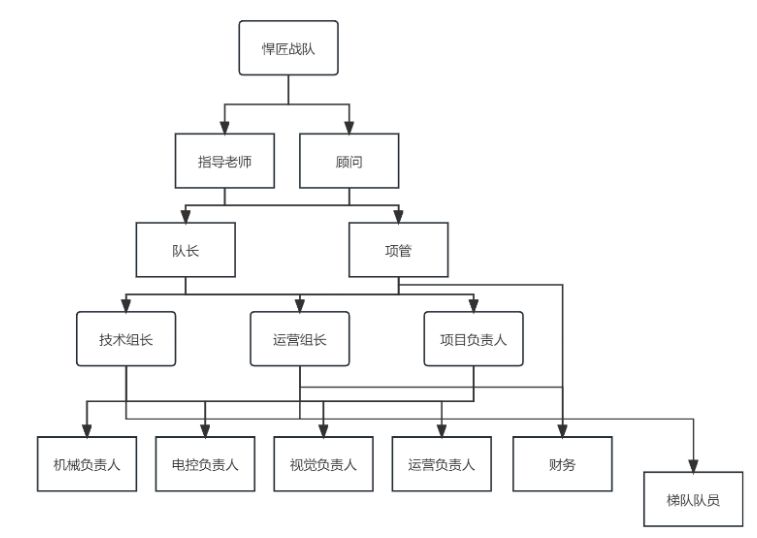
\includegraphics[height=0.9\textwidth]{figure/teamStructure_review.png}
                    \hspace{0.5em}
                    \caption{\textbf{\zihao{-4}\textbf{组织架构示意图}}}
                    \label{fig:teamStructure_review}
        \end{figure}

    \subsection{规章制度建设}

    \subsubsection{规章制度建设重点分析}

    \subsubsection{规章制度落地方案分析}

    \subsubsection{规章制度落地闭环分析}

    \subsection{文化建设}

    \subsubsection{战队文化建设}

        \noindent
        \LTXtable{\textwidth}{table/5.3.1_teamCulture_construction.tex}

    \subsubsection{赛事文化渗透}

        
    
    \newpage
    
    \section{宣传及商业计划}


    \subsection{宣传计划}
    
    \subsubsection{宣传目的}

        \setlist[itemize]{label=\raisebox{-1.2ex}{\scalebox{3}{$\textbullet$}}}

        \begin{itemize}
            \item 首先,悍匠战队宣传工作立足于提升悍匠战队的知名度和影响力。通过全方位的宣传策略,包括公众号推广、视频制作等,让更多人了解悍匠战队在RoboMaster赛事中的精彩表现及在团队协作方面的卓越能力。
            \item 其次,宣传也是凝聚团队内部力量的重要手段。通过宣传展示战队奋斗历程、历史成就和战队内核,能够激发战队成员的归属感和自豪感,增强团队的凝聚力和向心力,为接下来的比赛和团队发展注入源源不断的动力。
            \item 除此之外,宣传可以吸引更多志同道合的人才加入悍匠战队。宣传工作可以让他们看到悍匠战队的潜力和价值,从而吸引他们加入,共同为悍匠战队攀越高峰贡献力量。
        \end{itemize}

    \subsubsection{宣传人员要求}

        悍匠战队在参加RoboMaster赛事的荣耀征程中,深知宣传工作的重要性。因此,对于运营组宣传人员,战队设定了以下具体的要求:

        \setlist[itemize]{label=\raisebox{-1.2ex}{\scalebox{3}{$\textbullet$}}}

        \begin{itemize}
            \item 悍匠战队日常运营微信公众号、短视频平台等,宣传人员应具备出色的创意思维和一定的文字功底,对RoboMaster赛事充满热情,并将这种热情转化为感染力强的宣传内容,策划出新颖、独特且富有吸引力的宣传方案,撰写出富有感染力的文章及社交媒体文案。
            \item 另一方面,宣传人员还承担了团队周边制作、海报、视频剪辑等重任,熟悉视觉设计软件(如Adobe Creative Suite、Canva等),注重色彩搭配、布局设计及视觉冲击力,能够独立完成海报、宣传册、视频剪辑等视觉素材的制作,也是对宣传人员的要求之一。
            \item 尤其重要的是,宣传人员应具备良好的沟通能力与团队精神,能够与战队其他成员(如技术团队、指导老师等)有效沟通,共同策划并执行宣传计划。主动承担责任,对宣传工作抱有高度的责任心,确保每一项宣传任务都能按时、高质量地完成,确保宣传效果最大化。
        \end{itemize}

    \subsubsection{宣传方式}

        \setlist[itemize]{label=\raisebox{-1.2ex}{\scalebox{3}{$\textbullet$}}}

        \begin{itemize}
            \item 悍匠战队新媒体平台:微信公众号(悍小酱RoboMaster)、哔哩哔哩账号(悍小酱RoboMaster)、抖音账号(悍小酱RoboMaster)。
            \item 悍匠战队线上宣传途径:微信公众号推文推送、视频剪辑及其发布、海报与宣传册制作等。
            \item 悍匠战队的线下活动:宣讲会、社团嘉年华、海报发放、实验室参观交流、开放日等。
            \item 悍匠战队的对外宣传借助:学校官方微信公众号及学院官方公众号、机甲大师官方论坛等。
        \end{itemize}

    \subsubsection{宣传指标}

        \noindent
        \LTXtable{\textwidth}{table/5_propagandaIndex.tex}
    
    \subsubsection{宣传规划}

        \noindent
        \LTXtable{\textwidth}{table/5_publicityPlan.tex}
    
    \subsubsection{周边规划}

        \LTXtable{\textwidth}{table/5_giftPlan.tex}
        

    \subsection{商业计划}

    \subsubsection{战队招商客户规划}
    
    \subsubsection{战队招商资源优势及亮点}
    
    \subsubsection{战队招商目标规划}

    
    \newpage

    % 引入封底
    % 封底
    

\includepdf{section/cover2.pdf}

\end{document}
%%% 文档内容-END
%%% 文档内容是正文部分,我们只需编辑 ./section/ 目录下的文档即可